\documentclass{article}
\usepackage{graphicx}
\usepackage{hyperref}
\usepackage{float}
\renewcommand\textfraction{.1}
\title{ {2nd Partial Project}\\
        Introduction to Data Science\\
        Exploratory Analysis\\
        US airports’ delays and cancellation}
\date{2016-10-26}
\author{Ivan Soto\\
        Erick Ibarra}
\begin{document}
    \maketitle
    \pagenumbering{gobble}
    \newpage
    \pagenumbering{arabic}
    \section{Introduction}
    \subsection{Overview}
    This research is aimed to identify and select a question that arises in the US Delays
    and Cancellations domain. The purpose of this document is to present the
    problem statement, the question derived from it and the approaches that are
    going to be used to elicit an answer to this question. Description of the
    data and a descriptive analysis will be provided as well.
    \subsection{Problem Statement}
    An aviation startup company (Avinalytics) is about to launch a new project, in which they want to understand and characterize the delays and cancellations to create an app capable to determine the likelihood of a flight in the US being cancelled.

First, they want to analyze historical flight data and identify patterns and characteristics for the different flight delays and cancellations, based on the date, the airline operators, the airports, route structures, region or state of the country, etc. The Avinalytics company hires you to perform this task.

    \subsection{Motivation}
    It comes as no surprise that there are over 3000 commercial flights every day.
    As expensive as traveling through air can get, it is expected that this
    service will be flawless. A great number of people traveling through air anticipate
    the date they are planning to flight, most likely expecting their travelling
    experience will be smooth. Unfortunately, it can be seen that is not always
    the case: flights can be delayed or cancelled for several reasons, that end
    up disrupting the plans for a traveler.\newline
    \indent In order to aid people who often travel through air, the following question
    has to be answered: Given a flight, \textbf{is it likely to be cancelled?}

    \subsection{Approach}
    In order to answer this question, historical flight data has been downloaded
    from the Office of the Assistant Secretary for Research and Technology: Bureau
    of Transportation Statistics. Data delivered in this way is said to
    be secondary data, that for our research suffices to get close to answering
    our question.\newline
    \indent For every observation in the data set, the outcome of the flight is
    stated. This allows us to consider this problem as a supervised learning task,
    studied under the field of Machine Learning.
    To be more precise, there are two possible outcomes for each flight: cancelled
    or not cancelled. From now on, the terms "outcome" and "class" will be used
    interchangeably, the same goes for the terms "observation" and "training example".
    Since there are classes to which a training example can belong, this now becomes
    a classification problem. An algorithm that implements classification is known
    as a classifier. A classifier will allow us to tell, for any given example, the
    class to which it most likely belongs.\newline
    \indent With the purpose of selecting the
    classifier that best formulates a prediction function $f(x)$, the data has to
    be analyzed through descriptive and exploratory analysis to find patterns: the accuracy of a classifier is subject to
    the model the data most closely resembles. Once we suspect of a possible model,
    we train several classifiers by feeding them a training set in order to set
    them ready to make predictions for any example. Tuning a classifier is important
    to achieve better accuracy as well as trying several training sets
    to ensure that the model is not overfit to the data.
    \newpage
    \section{Descriptive analysis}
    \subsection{Introduction}
    Before anything else, basic features of the data in this study will be described, in order to
    provide simple summaries about the sample taken and get a better understanding of it. The data collected from the Bureau
    of Transportation Statistics contained eleven datasets, each of which contained at least 400,000 observations.
    Around 10\% of the dataset was sampled randomly for further analysis so as to quickly process it to present descriptive
    and exploratory statistics.
    For a classifier to work with higher accuracy, the subset of features that best represent
    the data aligned to the question to be answered has to be chosen. There are
    algorithms in the field of Machine Learning that reduce the dimensionality of
    the number of features, and that can result in overall improved accuracy.

    \subsection{Feature selection}
    Out of the 110 features available for each observation in the data set, a subset
    of those were selected as representative features through manual selection. The following
    gives a brief description of each of the features selected:
    \begin{itemize}
        \item Time Period
        \begin{itemize}
            \item Quarter\\
                Period of the year which can be related to seasonal changes.
            \item Month\\
                Period in time that can be related to vacations, trends or important
                 events.
        \end{itemize}
        \item Airline
        \begin{itemize}
            \item UniqueCarrier\\
                Identifier of the brand or airline that owns the flight can help
                identifying trends about the management of each airline.
            \item FlightNum\\
                Unique identifier from each flight which is ultimately the unique
                identifier for each observation.
        \end{itemize}
        \item Origin
        \begin{itemize}
            \item OriginAirportID\\
                Identifier from which the flight departed, can help to identify
                problems related to departure of specific locations or cities.
        \end{itemize}
        \item Destination
        \begin{itemize}
            \item DestAirportID\\
                Id of the airport the flight arrived to, it can be related
                to air congestion in given location or arrivals management.
        \end{itemize}
        \item Departure Performance
        \begin{itemize}
            \item CRSDepTime\\
                Computer Reservations System Departure Time refers to the time the
                flight is scheduled it may help to find problems related to specific
                 periods of time in the day.
            \item DepDelay\\
                The difference between the scheduled departure time and the actual
                 departure time of the flight it may help see a relation between
                 time loss and flight cancelations.
        \end{itemize}
        \item Arrival Performance
        \begin{itemize}
            \item CRSArrTime\\
                The computer calculated arrival time.
            \item ArrDelay\\
                Difference between the computer estimate and the actual time of
                arrival.
        \end{itemize}
        \item Cancellations and Diversions
        \begin{itemize}
            \item Cancelled\\
                The actual class the observation belongs to it can acquire
                the values of cancelled or not cancelled. This will be the value
                produced by the function $f(x)$ given an input flight and its
                conditions.
            \item CancellationCode\\
                Although this might not help to actually classify the data
                it can be used during the exploratory analysis to figure out
                the patterns which produce this type of cancelation.
        \end{itemize}
        \item Flight Summaries
        \begin{itemize}
            \item Distance\\
                Physical separation between the origin airport and the
                destination. It can help to guess problems related to air
                time, gas or mechanical issues.
        \end{itemize}
    \end{itemize}
    \subsection{Analyzing the features}
    For some of the features previously presented, statistics will be presented that may show interesting
    facts about the data, and which can further aid in the process to get a bit closer to answering our question.\newline
    Before analyzing the specific variables of the dataset, a summary of the the sample with the selected variables was done
    in order to observe some basic behaviors on the dataset.\newline
    \begin{figure}[h!]
      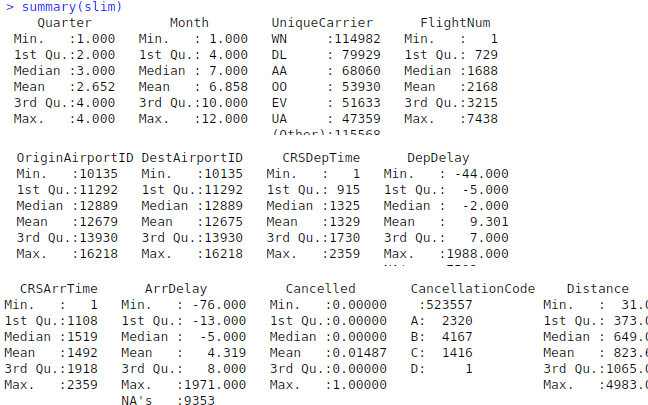
\includegraphics[width=\linewidth]{r_plots/summ.png}
      \caption{Dataset Summary}
      \label{fig:graph1}
    \end{figure}

    Starting from the feature named "Quarter", the most we can get out of it alone is the quarter in which most of the planes
    took plane. Figure 2 shows the number of flights registered in our sample for each of the quarter, and it can be seen
    that quarter 3 had more flights slightly over quarter 2.

    \begin{figure}[h!]
      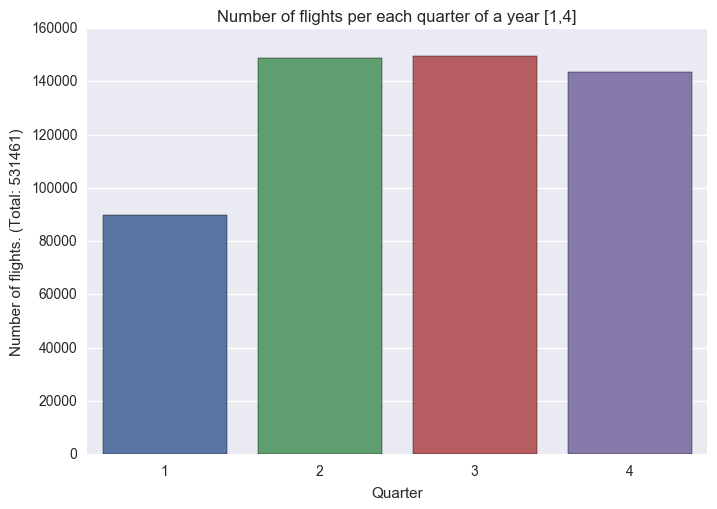
\includegraphics[width=\linewidth]{graph/quarter_flights.png}
      \caption{Flights per year quarter}
      \label{fig:graph1}
    \end{figure}
    % \newline

    It may prove interesting to show which flight numbers have been on the air the greater number of times. Figure 3 plots the
    occurrences of each flight number. It can be important to show
    at some point if this holds true: the more frequent a flight the more prone it is to delays, and the same analysis for cancellations, which is what the question seeks
    to answer. The mode ended up being flight number 469 with 376 appearances in the dataset.
    \begin{figure}
      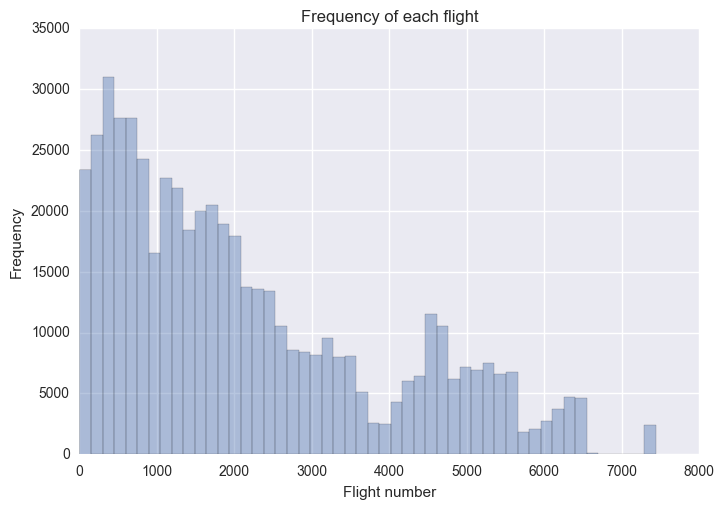
\includegraphics[width=\linewidth]{graph/flightnums_freq.png}
      \caption{Frequency of flights}
      \label{fig:graph1}
      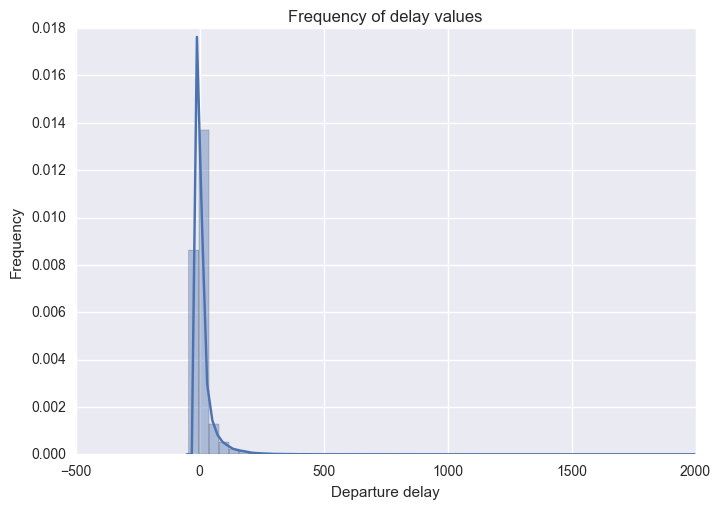
\includegraphics[width=\linewidth]{graph/delay_flights.png}
      \caption{Delay on flights}
      \label{fig:graph1}
    \end{figure}
    % \newline
    The same issue happens for the rest of the categorical variables: we can at most get the mode out of them at this point.

    How about non-categorial variables, such as departure delay? Since this is a continuous random variable, statistics such as the mean and the standard deviation
    can be obtained. A value of 9.3005 was found to be the mean for this feature, which means that on average, flights are delayed
    by slightly more than 9 minutes. It might be interesting to show, further in the study, how delay time affects the outcome of
    a flight. As for the standard deviation, 36.807 was calculated, reflecting the extent to which data is spread out with respect
    to delay time. If this were to be plotted, observations could be made about the continuous probability distribution that this data shows, as illustrated in Figure 4. As seen, the curve is clearly skewed to the right, and that could mean a plane rarely gets
    delayed for a long period of time.

    Distance is also a continuous random variable, and a plot can show the probability distribution it fits. Figure 5 shows this plot
    and no known distribution can be identified, except it looks skewed to the right. It can only be said that most flights do not
    travel really long distances.

    \begin{figure}[H]
      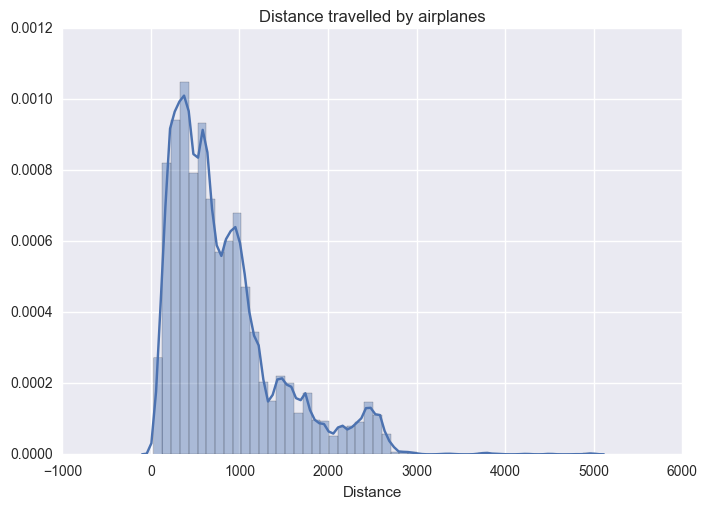
\includegraphics[width=\linewidth]{graph/dist_flights.png}
      \caption{Distance of flights}
      \label{fig:graph1}
      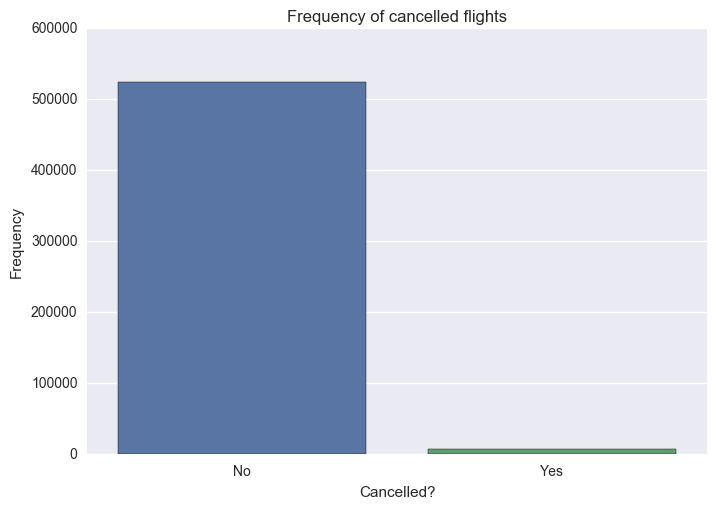
\includegraphics[width=\linewidth]{graph/cancelled_flights.png}
      \caption{Cancelled flights}
      \label{fig:graph1}
    \end{figure}
    
    Last but not least, statistics on the "Cancelled" feature. Figure 6 compares the number of cancelled flights to the number of not-cancelled flights. We can clearly see that the number of cancelled flights is really low! Based on this, we can tell with no
    precise numerical value that the probability of a flight being cancelled is low.

    In order to get a better view of the dataset, also, a boxplot for each numerical variable was plotted and only the interesting ones where chosen to be included in this document. This first boxplots in figure 7 are of all the numeric values in the set in order to see trends or to draw different conclusions. Some of the interestings include the distance boxplot which is shown on figure 8 and displays that most of the distances are in a range of less than 1000 km, so flights with great distances as shown previously are less common and may bring more problems such as being delayed a lot of time or even being cancelled. 

    \begin{figure}
      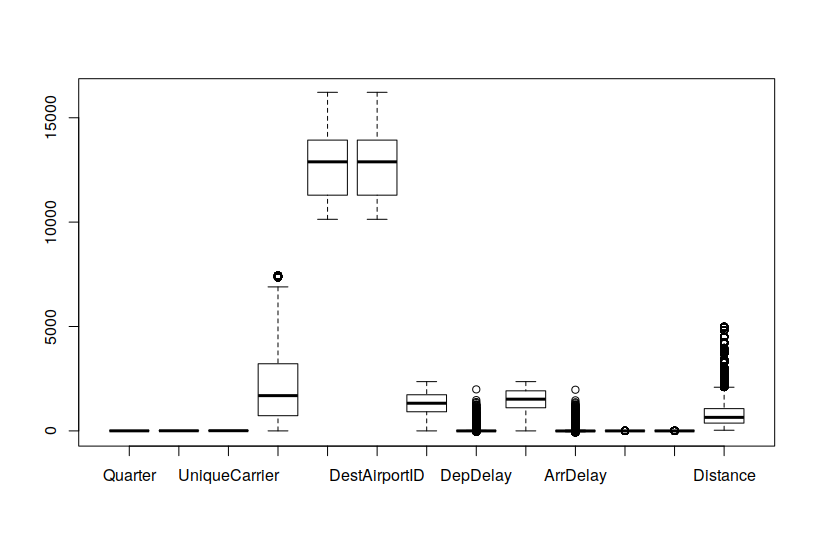
\includegraphics[width=\linewidth]{r_plots/boxes.png}
      \caption{Slim Dataset}
      \label{fig:graph1}
      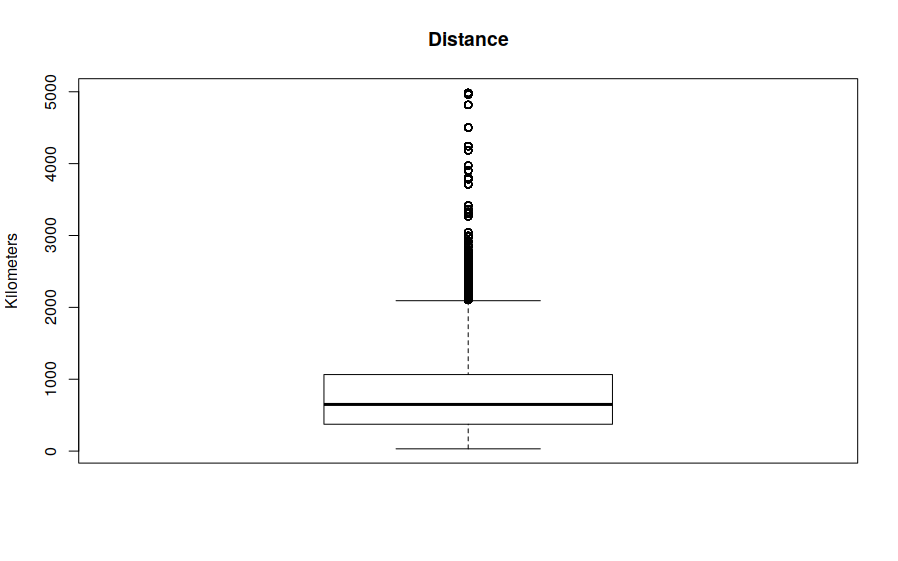
\includegraphics[width=\linewidth]{r_plots/box_distance.png}
      \caption{Distance Boxplot}
      \label{fig:graph1}
    \end{figure}
    % \newline

    Other interesting boxplots where the ones related to the delay, but we will only take a look at the departure delay, since both the arrival and departure delay behave in a similar manner. As we can see, the majority of the flight with delay didnt take much delay. The median of the set is around the negative delay, so most of the flight arrived early to make the connection, but there are also a lot more that took over 15 minutes all the way up to a 2000 minutes of delay which given the circumstances we cant say it is an outlier.\newline
    Some other information can be retrieved if we take a look at the boxplots given by the delay by each carrier which we can observe in the figure 11 and in figure 12 a boxplot which separates the delays by each motive of cancellation.

    \begin{figure}[H]
      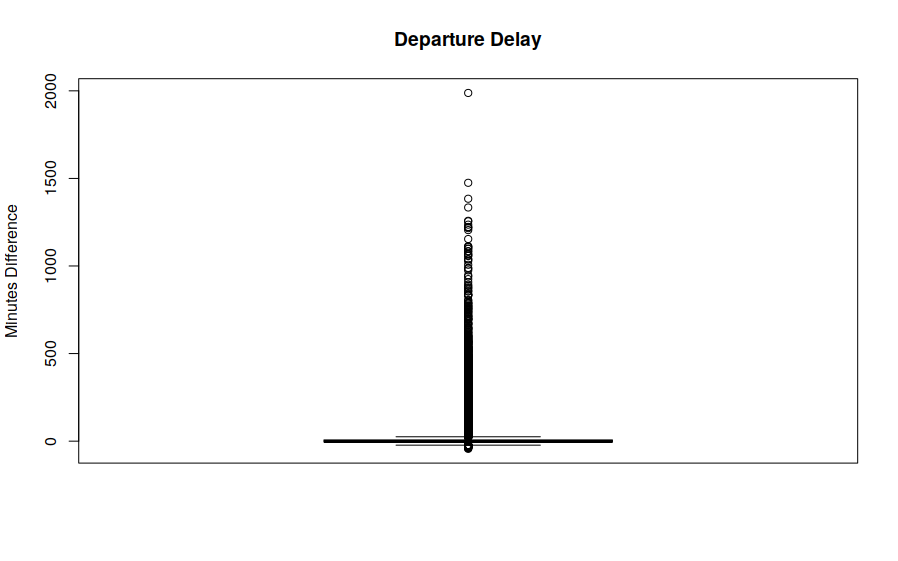
\includegraphics[width=\linewidth]{r_plots/box_dep_delay.png}
      \caption{Departure Delay}
      \label{fig:graph1}
      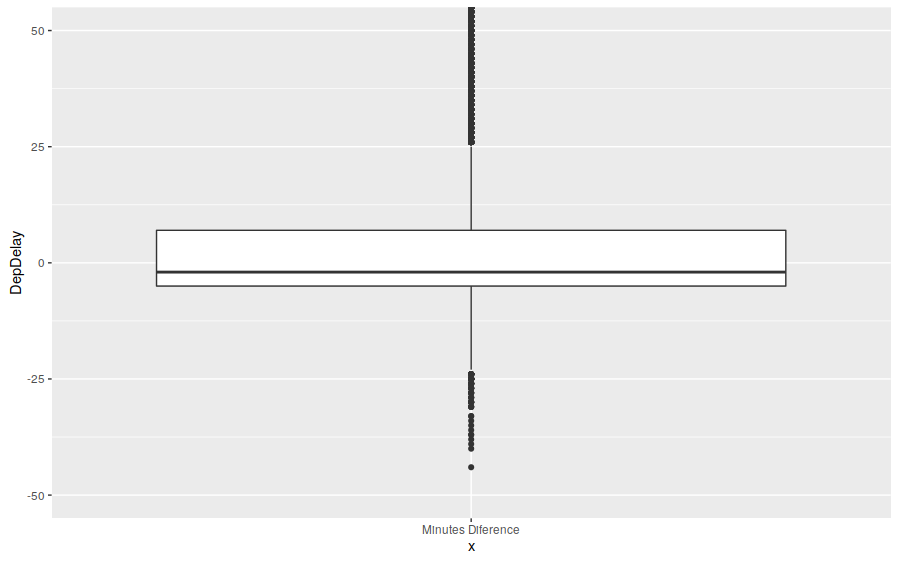
\includegraphics[width=\linewidth]{r_plots/box_dep_delay_zoom.png}
      \caption{Zoomed Departure Delay}
      \label{fig:graph1}
    \end{figure}

    \begin{figure}[H]
      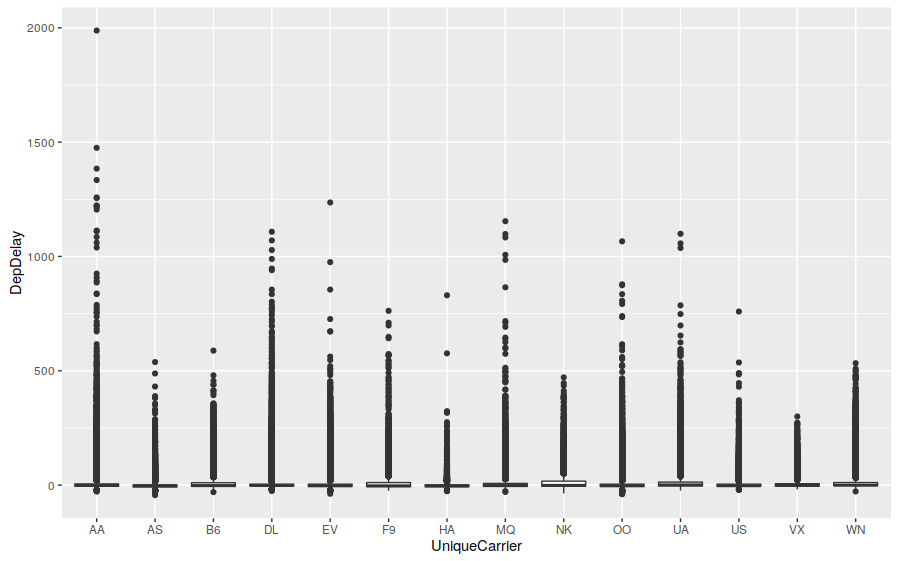
\includegraphics[width=\linewidth]{r_plots/box_delay_by_carrier.png}
      \caption{Zoomed Departure Delay By Carrier}
      \label{fig:graph1}
      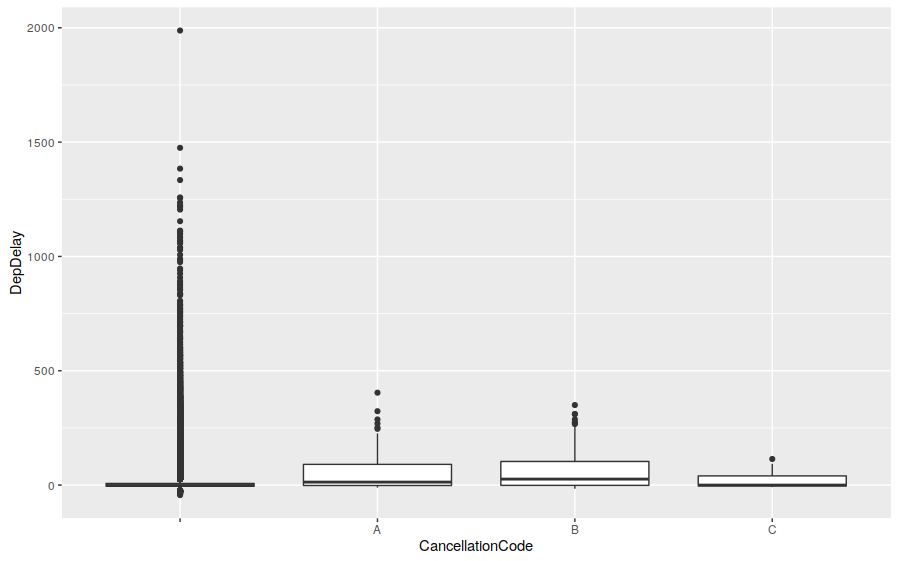
\includegraphics[width=\linewidth]{r_plots/box_dep_delay_by_code.png}
      \caption{Delay by Cancellation Code}
      \label{fig:graph1}
    \end{figure}


    \newpage
    \section{Exploratory Analysis}
        In order to see how the variables relate to each other and draw better conclusions we plotted all the variables against each other in a scatter matrix, but due to the sample being a bit on the big side, it was decided to separate the variables in 2 categories, one category related with time (Figure 13) and the other with places or airports (Figure 14). The one related to places since most of them are ids it really doesnt show any trend or relevant relation. But if we put our attention to Figure 13 the one related with time, we can start to see some trends on the dataset. For example, we can see how one variable behave given a change in the other variable, the most notorious example of this, is the CRS times against each other it was expected that they had a linear relation as the delay times had, but there is an interesting spot which could generate other cluster and could mean different things. Other of the most relevant information obtained from the scatters, is how the cancelled variable relates to the other, for example, we can se how some spots of the cancelled flag against the distance or delays are empty, meaning most of the flights under those circumstances doesn't get cancelled.\newline
        Figure 15 shows the covariance and pearson correlation indexes of the variables plotted on Figure 13. Some of the interesting bits of this figure are that the most related variable to the cancelled one is the flight number with a index of 0.037 which is very low, so we cannot try to identify a main cause for the cancelation of a flight. After it, the most positively correlated variable is the departure time managed by the system. It is interesting to note that the distance shows a negative correlation index given if a flight is cancelled or not. Other information we can take is what we expected, that the most related columns of the dataset are the departure and arrival times by the CRS.

    \begin{figure}[H]
      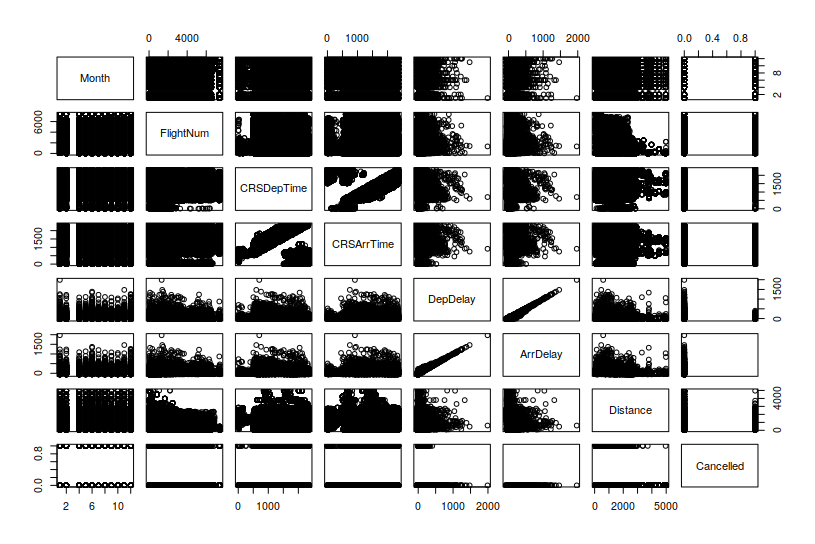
\includegraphics[width=\linewidth]{r_plots/times_matrix.png}
      \caption{Scatter Matrix Time Related}
      \label{fig:graph1}
      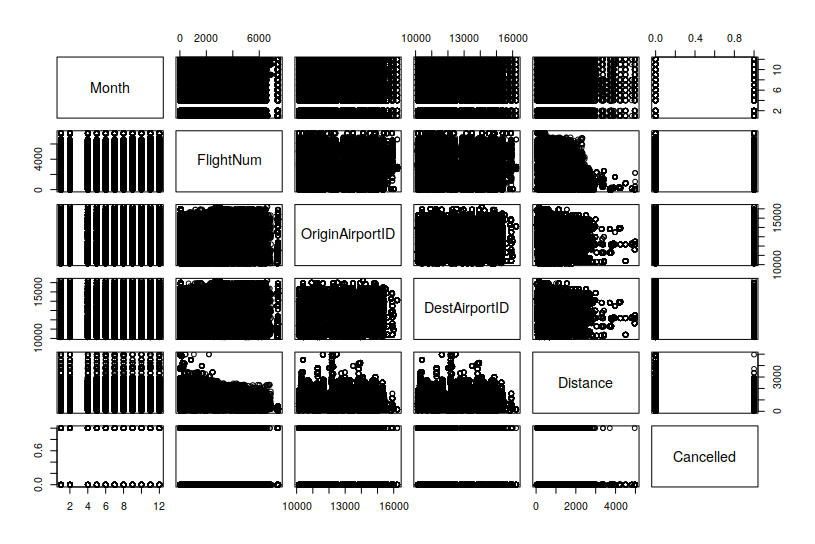
\includegraphics[width=\linewidth]{r_plots/destinos_matrix.png}
      \caption{Scatter Matrix Place Related}
      \label{fig:graph1}
    \end{figure}



    \begin{figure}[H]
      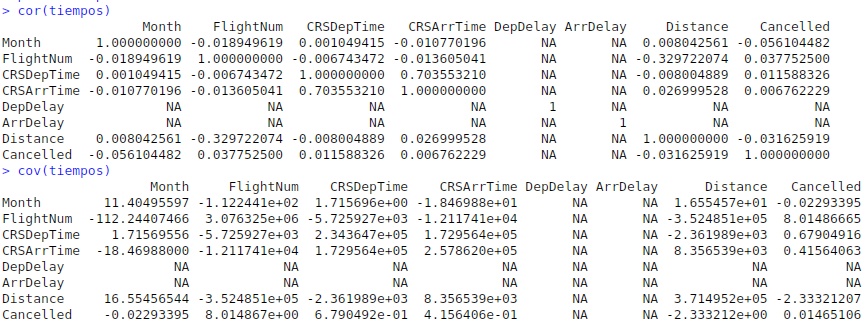
\includegraphics[width=\linewidth]{r_plots/cor_cov_times.png}
      \caption{Correlation and Covariance of Time Related Variables}
      \label{fig:graph1}
    \end{figure}

    \subsection{Plots}
    The variables in which we suspect some relations exists are plotted and presented in the next figures:\newline
    
    \begin{figure}[H]
      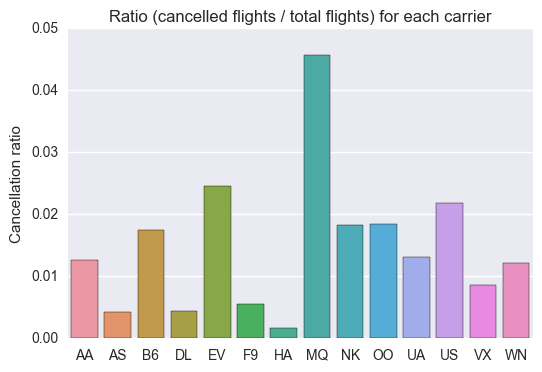
\includegraphics[width=\linewidth]{graph/ratio_cancelled_total.png}
      \caption{Ratio of cancelled flights on total flights based for each carrier based on
      historical data}
      \label{fig:graph1}
    \end{figure}
    The main causes for flight cancellation and delay are the following: air carrier delay,
    security delay, National Aviation System Delay and extreme weather\newline
    \indent The cause that is the easiest to analyze is air carrier delay. This is because
    the data does not have to be manipulated extensively to figure out how many cancellations
    have ocurred per air carrier. In Figure 16, it can be seen the ratio $(flight cancellations/total flights)$
    for each of the carriers for which there is data.\newline
    \indent We also suspect that for flights where long distances are travelled, it might influence
    on how much preparation is required before a flight, i.e. aircraft maintenance, crew
    availability, weather conditions, etc. It can be appreciated from Figure 17 that the
    flights with longer distances are most likely not to be cancelled. Based on this visualization,
    it can be concluded that distance is not probably an important cause for flight
    cancellation.
    \begin{figure}[H]
      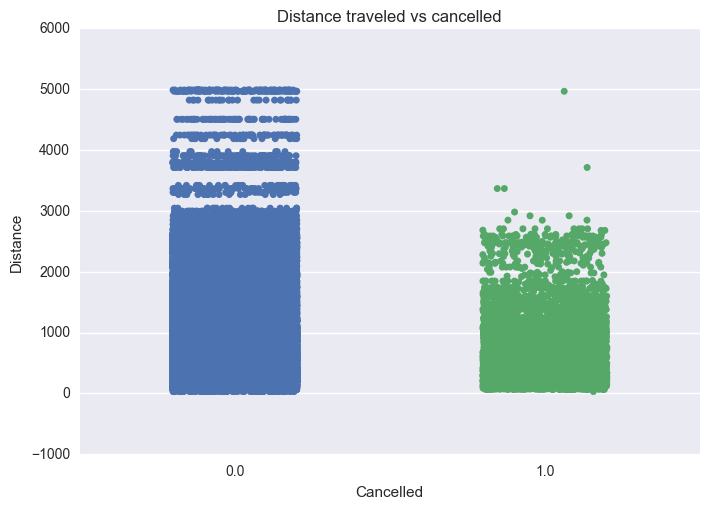
\includegraphics[width=\linewidth]{graph/ratio_cancelled_distance.png}
      \caption{Distance traveled (in miles) for each flight and its outcome (cancelled or not cancelled)}
      \label{fig:graph1}
    \end{figure}
    % \newline
    \indent It was also suspected that, the more delay a flight gets, there is a higher chance it might
    be cancelled. For this reason, the scatterplot shown in Figure 18 illustrates whether this
    holds true.
    \begin{figure}[H]
      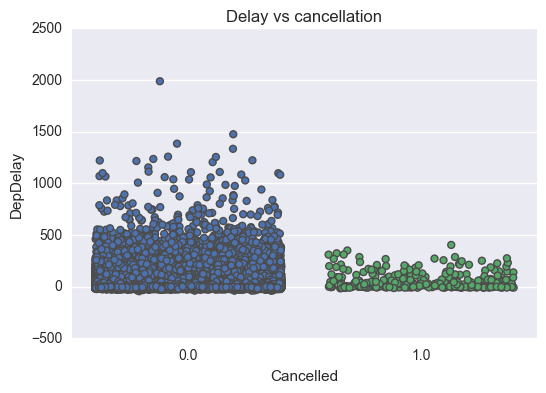
\includegraphics[width=\linewidth]{graph/ratio_cancelled_depdelay.png}
      \caption{Departure delay (in minutes) for each flight and its outcome (cancelled or not cancelled)}
      \label{fig:graph1}
    \end{figure}
    % \newline
    \indent Let's also recall some of the possible correlations that were superficially mentioned in the descriptive analysis section. It's important to analyze if any of the next scatterplots can show us any patterns in the data which can make answering our question easier. To start off, let's find out if a quarter has anything to do with the number of delays. Figure 19 depicts this comparison: it's seen that even if quarter 3 had the highest mode as shown in the descriptive analysis section, it can be appreciated that delays (at least for long delays) are more frequent in the other quarters, so even if quarter 3 has lots of flights, not every flight is delayed by a considerable amount of time (recall the mean was a bit more than 9 minutes).

    \begin{figure}
      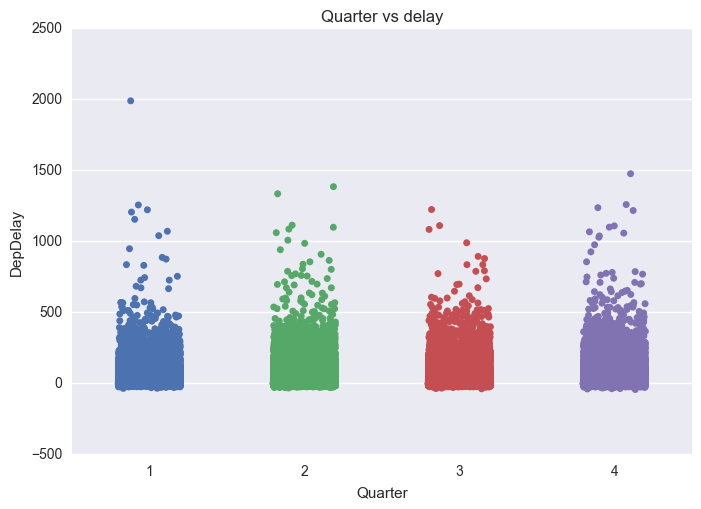
\includegraphics[width=\linewidth]{graph/quarter_vs_delay.png}
      \caption{Quarter vs delay}
      \label{fig:graph1}
      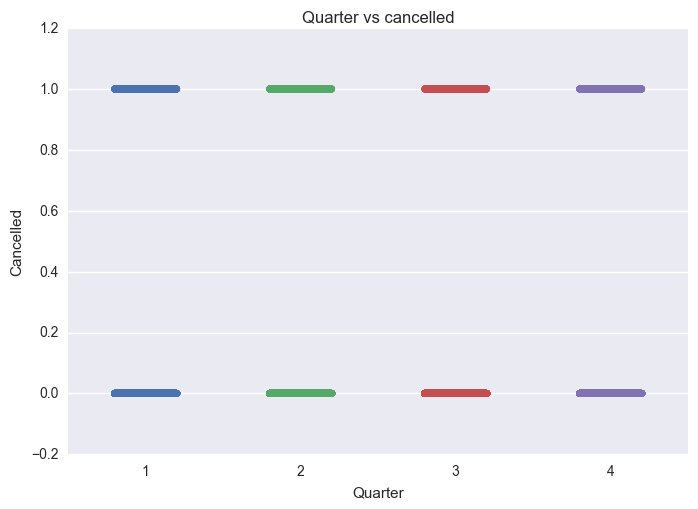
\includegraphics[width=\linewidth]{graph/quarter_vs_cancelled.png}
      \caption{Quarter vs cancelled}
      \label{fig:graph1}
    \end{figure}
    % \newline

    Now, there's a chance that in quarter 3 the number of cancellations was greater than in other quarter. Figure 20 shows similar results for all the quarters, and it's difficult to see differences between the four, but assuming that quarter 3 was indeed smaller in cancelled flights than the rest of the quarters, it can be said that the greater the number of flights on a given period does not correspond to a bigger number of cancellations, and this could possibly mean this: the period does have an impact on the performance of flights? In that case, quarter 3 is a good time to travel, because even if lots of flights took place during that time, other quarters shown more cases of delayed flights.\newline




    % \newline
    %
    % It's helpful to also see if certain flight numbers have some tendency to being delayed. Figure 11 illustrates the data for these two features correlated.
    %
    % \begin{figure}
    %   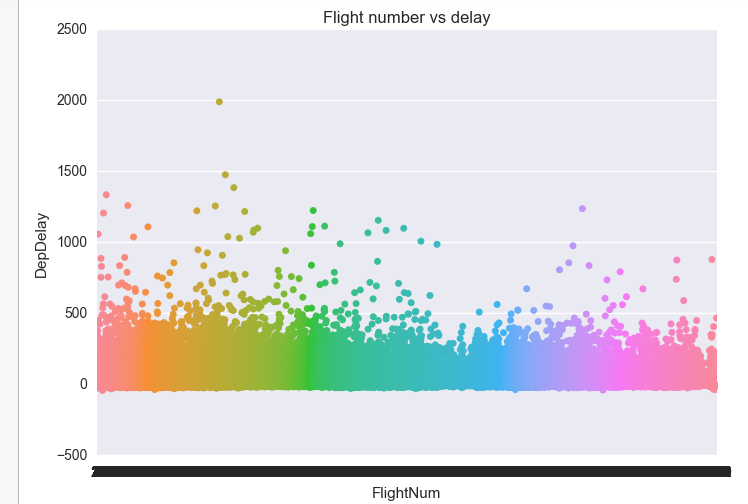
\includegraphics[width=\linewidth]{graph/flightnum_vs_delay.png}
    %   \caption{Quarter vs cancelled}
    %   \label{fig:graph1}
    % \end{figure}\newline

    \section{Conclusion}
    During the analysis, some of the hypothesis we had regarding possible correlation between
    a pair of features did not hold true as expected. Using elementary statistics techniques,
    we were able to reveal some of the features that weight in at identifying possible
    flight cancellations on the basis of problems due to internal carrier administration.\newline
    Answering this question is important now for one more reason: causes might not be those
    that we initially believed in. We might need a different insight to figure out how to
    find more significant patterns in the data. Up to this point, visualization of data
    only took place, and the next step is to try various classifiers, once more significant patterns
    have been found, feed them data, and understand their behavior and measure their accuracy.

    \section{Appendix}
    The code for the descriptive and exploratory analysis can be found in this repository: \url{https://github.com/IvanAli/DataScienceITESM}
    \section{Bibliography}
    On-time flights (2016). Document retrieved from Flight stats on September 15th, 2016 from: \url{http://www.transtats.bts.gov/DL\_SelectFields.asp?Table\_ID=236\&DB\_Short\_Name=On-Time}\newline\newline
    Flight delay cause (2016). Document retrieved from Flight stats on September 15th, 2016 from: \url{http://www.transtats.bts.gov/ot\_delay/ot\_delaycause1.asp?type=21\&pn=1}\newline\newline
    Flight Stats Global Cancellation and delays (2016). Document retrieved from Flight stats on September 15th, 2016 from: \url{http://www.flightstats.com/go/Media/stats.do}\newline
\end{document}
